\documentclass[12pt]{article}
\usepackage{amsmath}
\usepackage{graphicx}
\usepackage{subcaption}
\setlength{\parindent}{0pt}
\setlength{\parskip}{10pt} % block paragraphs
\usepackage{hyperref}
\usepackage{bm}
\begin{document}

\title*{\centerline{{CAP 5619 \-- Deep and Reinforcement Learning term
project}}}
\author*{\centerline{Hua Huang}}%unnumbered centered head

In this project, Reinforcement Learning is used to play the Atari
game of Pong \cite{15atari}. Since most of the efforts in the
literature are in the direction of CNN+Q learning, and we know that Q
learning plus bootstrap plus non\--linear function approximation is
inherently unstable. So all the algorithms based on DQN and the
original DQN paper have to tackle the instability by some carefully
designed techniques. For example, in the 2015 Nature paper \cite{15atari},
a separate target network is used in addition to the typical $Q$ network.
While the SARSA is on\--policy algorithm, 
and is inherently much more stable then Q\--learning. So it will be
worthwhile to try how SARSA performs in playing this game.\\

Linear function approximation will be considerred in addition to
Neural Network here. Linear function approximation based on Fourier basis
\cite{11fourier} will be implemented here. Fourier basis is
mathematixally appealing with its solid math ground. Any function can
be approximated with fourier basis.

\section{Introduction of game Pong}
Environment of Pong from module of Gym is adopted here for the Reinforcement
Learning. Gym is an open sourced package specially designed for RL
problems. In the ATARI simulators, the environment take the action
chosen by the algorithm, the the simulator will feed back the reward
and the information of next state.\\

In the game of Pong, agent manipulate the green paddle to bounce back the
ball, and are supposed to be able to discover techniques by itself to
win the game. Whenever the agent or the opponent acheieves 21 points,
an episode is done. The reward will be $1$ when the opponent miss the
ball and be $-1$ when the agent miss the ball, and $0$ otherwise. The
state is the RGB values of the screen. To facilitate the shawllow
function approximation, which is feasible only for small dimensions,
the positions of the ooponent, ball, and agent is extracted. Namely
instead of the end\-- to\-- end trainning, the agent has access to the
objects of the game. The actions are $\{NOOP, UP, DOWN\}$, in which
$NOOP$ will do nothing to the agent paddle. In the game design, the
agent paddle has a huge momentum effect, namely the velocity
impacts the action effect significantly.
\begin{figure}[h]
    \centering
    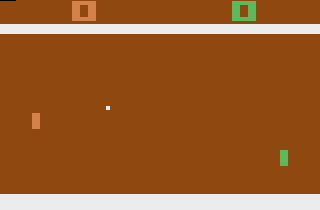
\includegraphics [scale=0.5]{pong.png}
    \caption {Game of Pong}
\end{figure}

\section{Reinforcement Learning system}
To overcome the partial observability, $3$ consecutive (not exactly
consecutive, since frame skip of 4 is used here, during the frame
skip, the same action is carried out 4 times, and the feed back will
be the final state and the reward will be the sum of the rewards
colelcted durin gthese 4 time steps) frames are recorded. By
inspection, we can see that the ball always travel $\pm 2$ in
horizontal direction, and the once get bounced back by the paddles or
by the upper/lower wall, the vertical velocity never changes
magnitude. Only the agent paddle has momentum effects. In this study,
we neglect the opponent position effects, namely we just focused on
the agent paddle and ball. Overall, the state is designed as
\begin{equation}
    \bm x_t=[v_{t-1}^b, x_t^b, y_t^b, v_{t-2}^a, v_{t-1}^a, y_t^a]
\end{equation}
in which $b$ stands for ball, $a$ stands for agent paddle, and 
\begin{equation}
    v_{t-i}^a=y_{i+1}^a-y_i^a, i\in\{1,2\}
\end{equation}
As the state indicates, we keep 3 frames for paddle agent to alleviate
the partial observability. In comparison, in DQN\cite{15atari}, 4
consecutive frames are used.
\subsection{Linear function approximation}
With linear function approximation, the features are constructed as 
\begin{equation}
    \phi_i(\bm{x})=cos(\bm{c_i} \cdot \bm{x})
\end{equation}
in which $\bm x$ is the normalized state, namely
\begin{equation}
    \phi(\bm{x})= \frac{\bm{x}-\bm{x_{min}}}{\bm{x_{max}}-\bm{x_{min}}}
\end{equation}
and $\bm{x_{max}}$, $\bm{x_{min}}$ are got by observing 1 million
frames off\--line. $\bm{c_i}$ is a 6\--dimensional vector with
components $c_i[j]\in[0, 10]$ for $j\in \{0, 1, 2\}$, and  
$c_i[j]\in[0, 5]$ for $j\in \{3, 4, 5\}$. Overall, there is
$11^3\times 6^3=287496$ features. \\
Since the horizontal velocity is always $\pm 2$, we can utilize this
binary nature by designing separate weights for the ball moving left
and moving right. Since there are $3$ actions, overall, we have
$2\times3\times 287496=1724976$ weights.
\subsection{Multilayer Perceptron}
In the neural network version of function approximation, a MLP is
used. In which there are 4 hidden layers with 256 units, one output
layer with single unit, overall, there are 
$2\times3\times(7\times256+3\times257\times256+257)=1591302$
weights. ReLU is used here. The weights in the kernel are initialized
following a standard normal distribution, and divided by the square
root of 256. The bias units are initialized as 1. 
\subsection{$SARSA(\lambda)$ algorithm}
$SARSA(\lambda)$ algorithm is a combination of the $SARSA$ algorithm with
eligibility traces\cite{18sutton}. Basically, eligibility traces is
similar to the momentum, and it's a backward view. Each update based
on the current TD error combined with the current eligibility traces
of past events:
\begin{equation}
    \bm{\omega}_{t+1}=\bm{\omega}_t+\alpha \delta_t \bm{z}_t
\end{equation}
in which the TD error:
\begin{equation}
    \delta_{t}=R_{t+1}+\gamma \hat{q}(S_{t+1}, A_{t+1}, \bm \omega_t)-
                              \hat{q}(S_{t},   A_{t}, \bm \omega_t)
\end{equation}
and the action\--value form of the eligibility trace:
\begin{eqnarray}
    &\bm{z}_{-1}&=0 \nonumber\\
    &\bm{z}_{t}&=\gamma \lambda \bm z_{t-1}+
                 \bigtriangledown \hat q(S_{t},   A_{t}, \bm \omega_t)
\end{eqnarray}
In this study, discount $\gamma=0.95$, $\lambda=0.95$. 

\section{Results}
The average rewards are given in Fig.2 for linear function
approximation.
\begin{figure}[h]
    \centering
    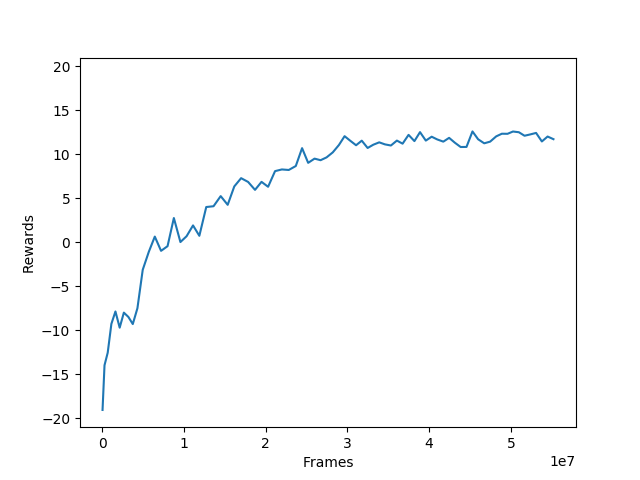
\includegraphics [scale=0.5]{rewards.png}
    \caption {Rewards}
\end{figure}
In this figure, the rewards are averaged over 100 consecutive episode,
the final socre is about $12.6$, and it seems it stops learning.
In comparison, the original DQN result is 18.9. We can see there is
still a large performance difference. In addition, state ot the art of
linear function approximation in solving Pong is 20.2\cite{16liang},
and in which a tremendous number of 114702400 features are used! The
professional human player can score 9.3\cite{15atari}. So it is better
then human, but worse then state of the art.\\
To improve the performance here, an manuel inspection of the decision
makings are carried out, quite superisely, to a large extent, the
agent will miss the ball after the paddle take an exploration step,
especially when the ball is approaching the paddle. Durin gthe last
few steps, any exploration action can potentially leads to a
catestrophic disaster. It is reasonable to speculate decreasing the
exploration rate will alleviate this effect. So a new experiment is
carried out here: Instead of a fixed $\epsilon=0.05$ (except for the 
first 100000 frames, during which $epsilon$ is decreased using a quotiant
function from 1 to 0.05). After 4500 episodes, the exploration rate is
halved every 500 episodes. The new result is given in Fig.3.
\begin{figure}[h]
    \centering
    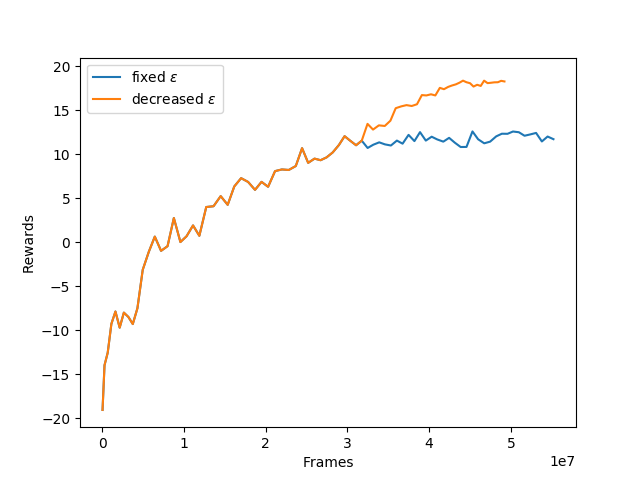
\includegraphics [scale=0.5]{rewards1.png}
    \caption {Rewards}
\end{figure}
This time the average rewards increased significantly, it acheives a
final score of $18.4$, which is about the same level as the much
sophisticated DQN! An animation of the trained agent playing the game
of Pong can be found here: \url{https://youtu.be/OeS_BPZslmM}\\

Due to time limit, the MLP $SARSA(\lambda)$ is still running, and the learning
curve is given in Fig.4. It achieved an average score about $-11$ after 12 
million frames. In comparison, after 12 million frames, LFA can achieve about 2.
It's safe to conclude that $SARSA(\lambda)$ with MLP approximation works. 
It is also possible to improve the results with finer tunning.
\begin{figure}[h]
    \centering
    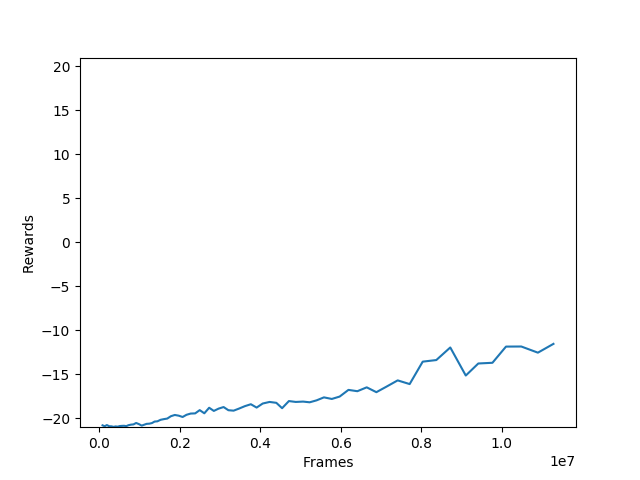
\includegraphics [scale=0.5]{rewards_mlp.png}
    \caption {Rewards with MLP function approximation}
\end{figure}

\section{Conclusion and future work}
Linear function approximation using Fourier basis can be utilized to
solve the game of Pong and acheived almost state\--of\--the\--art
result (The algorithms based on DQN keep evolving!). The experiment
also indicates blind exploration might lead to a disaster. A
straightforward related scenario is the application of RL to
self\--driving vehicles, in which safety is the top priority, and any
mistake can lead to life\--threaten consequences. Definitely a more
sophisticated exploration strategy should be incorporated. A future
direction is to design an algorithm enhanced by \textit{safe}
exploration. One of the approachs might be learn a local model for the
agent, and in decision making, we look forward a few steps and omit
the choices which are predicted to lead to failng scenarios. This work is
currently underway.

\begin{thebibliography}{9}
    \bibitem{15atari}
        Mnih, V. et al. \textit{Human-level control through
        deep reinforcement learning}.Nature 518, 529-533 (2015).

    \bibitem{11fourier}
         Georgia Konidaris et al. \textit{Value Function Approximation in 
                        Reinforcement Learning using the Fourier Basis},  
                        AAAI, 2011.
    \bibitem{18sutton}
         Richard S. Sutton and Andrew G. Barto, \textit{Reinforcement
         Learning: An Introduction}, The MIT Press, 2018.

     \bibitem{16liang}
         Yitao Liang et al., \textit{State of the Art Control of Atari
         Games Using Shallow Reinforcement Learning}, AAMAS, 2016.
\end{thebibliography}

\end{document}
